\title{G54FUZ Coursework Report}
\author{
  Jack Ellis \\
  psyje5@nottingham.ac.uk\\
  4262333\\\\
}
\date{}
\documentclass[12pt, a4paper]{report}
\usepackage{graphicx}
\graphicspath{{../}}

\usepackage{listings}
\lstset{
  basicstyle=\fontsize{9}{11}\ttfamily
  ,breaklines=true
}

\begin{document}
\maketitle

\tableofcontents

\section{Description of The Problem}

The task given is to create a fuzzy inference system (FIS) which will, given a patient's temperature and perceived headache, return a value representing "how much they need to go to the hospital".
This is to say the value returned will describe, out of 10, the potential severity of any medical condition and the priority they should give to making a trip to the nearest medical practise.

\par

To assess the quality of the FIS I will be looking at the control surface and, as the FISes become more complex, calculating the root-mean-square error for a more precise view of the difference between the desired output and the real output.

\par

The desired output of the system is a function whose control surface resembles the end of a valley, with 0 headache and a temperature of 37 resulting in an urgency of 0, any headache of 10 resulting in an urgency of 10, and a temperature of either 35 or 37 resulting in an urgency of 10.

\subsection{Gathering Membership Functions and Terms}

The first step was to gather the terms for the input variables, and generate appropriate membership functions.
I initially chose 5 membership functions per variable, input and output, given that for temperature and headache I was working with ranges of 4 and 10 respectively.

\subsubsection{Temperature}

I used the NHS website's guidelines on hypothermia for this; it states that normal body temperature for an adult is 37 degrees C, and a person is in a state of hypothermia if their body temperature drops below 35 degrees C.
They do not have a source on hyp\textbf{er}thermia, however I believe it is reasonable to infer that it sets in at the same difference above normal body temperature, i.e. at 39 degrees C.

\par

I opted for Gaussian membership functions for temperature; these are good representations of biological functions due to their bell shape.
All of these functions have standard deviation of 0.5, and their centers are each degree within the range 35-39.

\subsubsection{Headache}

For the headache input variable I opted for a scale, 1-10, because the amount of pain a person is in cannot really be measured objectively.
Additionally there exist a number of 1-10 headache scales.
I again opted to use the NHS standard scale, specifically the one in Figure \ref{fig:painscale}

\begin{figure}[ht]
  \centering
  \caption{The pain chart used by the NHS}
  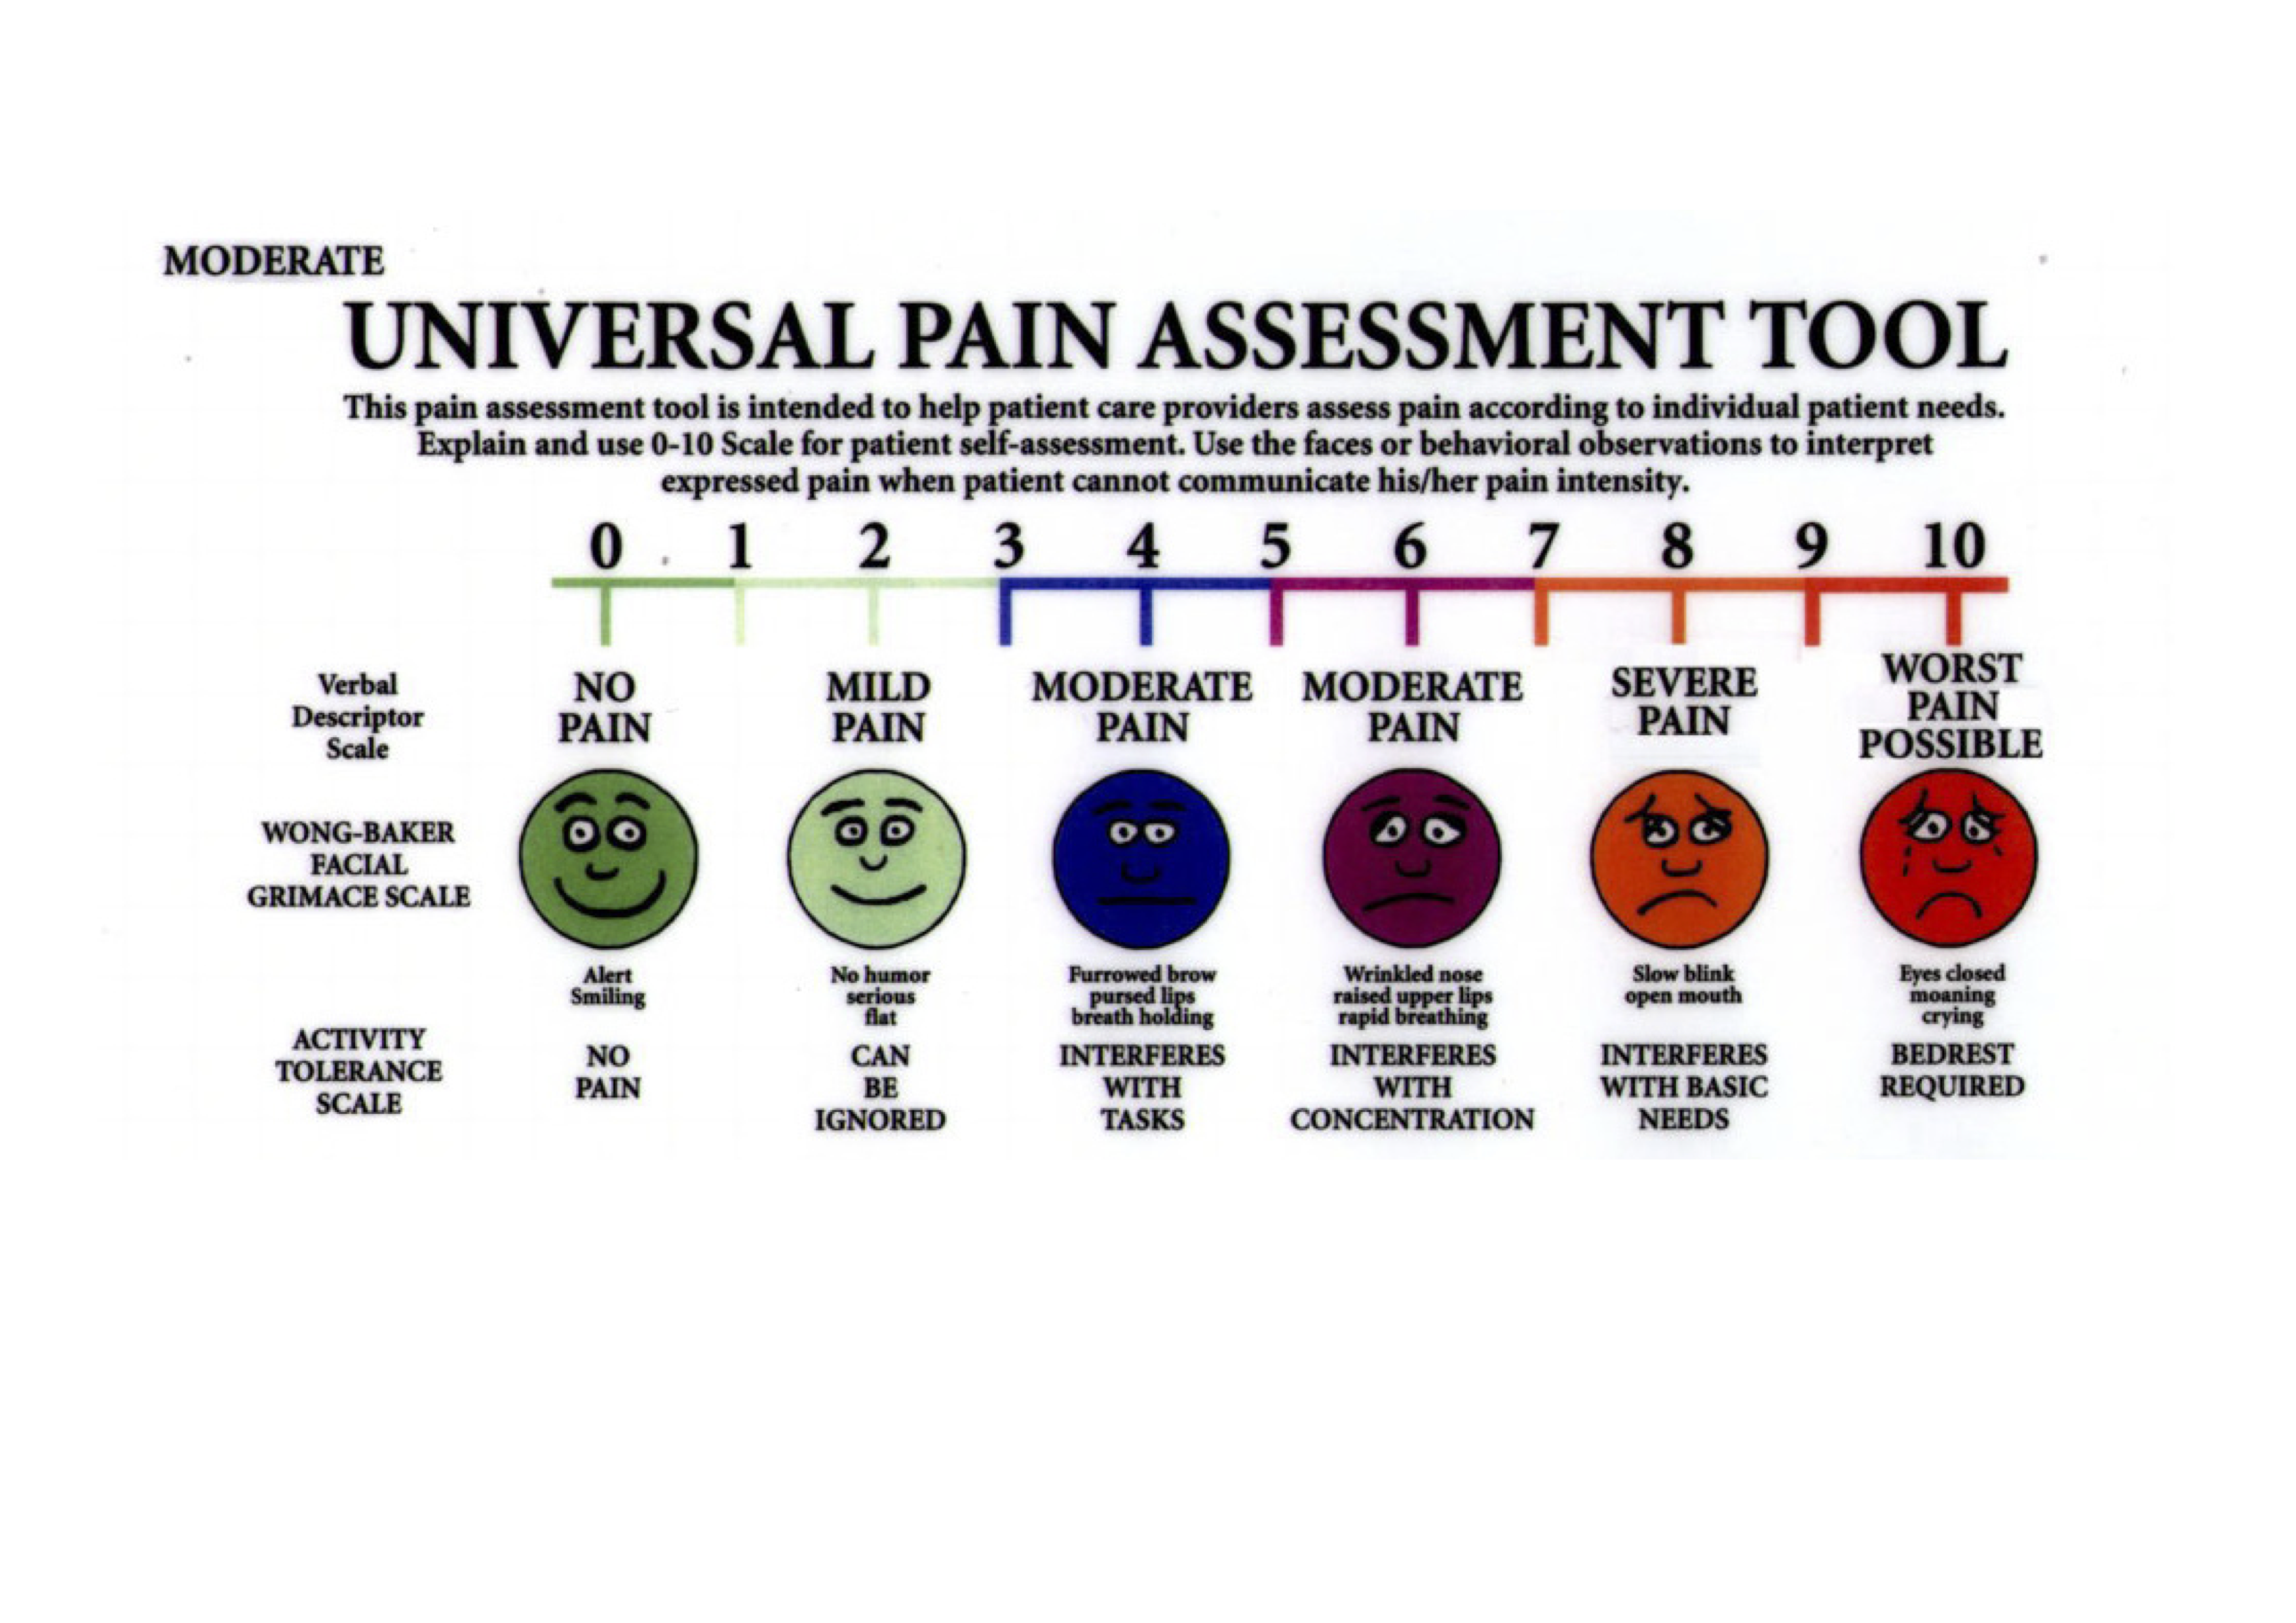
\includegraphics[width=\textwidth]{Report/Images/faces_scale_tool.png}
  \label{fig:painscale}
\end{figure}

\par

I chose trapezoidal membership functions initially, with each "section" of the chart making up the top of the trapezoid.

\subsection{Urgency}

This is on a scale of 0-10, with 0 being a perfectly healthy adult and 10 someone who will likely die if they are not immediately admitted to A\&E.
I consider someone at or under a rating of 3 someone who will likely be alright with some painkillers, and someone at or above an 8 to be a priority patient at A\&E. The 3 stages in between can be normally distributed.

\section{Description of Alternative Fuzzy Models}

\subsection{Individual Inputs}

The first 2 FISes I created used only the individual input values.
These were used as a baseline and to familiarise myself with the syntax and structure of creating a FIS in R.
For temperature the FISes control surface should resemble a valley, and for headache it should be a more or less straight upwards hill.

\subsection{Naively Combining The Terms}
The third model simply contained the two rulesets for the above models, without any further modification.
Its rules can be found in the appendix.

\subsection{A More Intelligent Combination}

This FIS combines the above rules in a more intelligent way, using OR and AND combinators to prevent the "valley" effect seen in Figure \ref{fig:membershipfns3}.

I consider this FIS to be at a point where the rules provide a good foundation for an inference system.
From this I created a further 5 FISes each with a difference defuzzification method, and one more with a different inference method.
At this point I began to use RMSE as an evaluation tool, with the defuzzification method \emph{Small of Maxima} providing the lowest RMSE (~1.50) however the control surface reduced the urgency at the absolute extremities, which is not acceptable behaviour in my view.

\par

The final modification I made to FIS 4 was to change the membership functions for the \textit{headache} from trapezoidal to Gaussian, in line with the membership functions for the other two variables.
With no other modification to the ruleset the control surface was much improved, with a smooth continuous increase of urgency.
The RMSE value for this is 1.56 which, while greater than that for FIS 6, is still less than that for the original FIS 4 on which the final model is based.

\section{Detail of Final Fuzzy Model}

The final FIS has 3 variables, for input headache and temperature, and for output urgency.
All 3 have 5 Gaussian membership functions, with the functions for the temperature being evenly spread and the ones for both headache and urgency having a very large "lower" function and a more compressed upper range.
It has an RMSE of ~1.56 and a continuously increasing control surface, which I believe to be the best compromise of these two evaluation methods.

\section{Discussion of Final Fuzzy Model}

The final model does provide - in my view - the best performance of the 11 FISes I created, but it is not perfect.
The control surface dips below the maximum urgency value for 10-rated headaches between temperatures of 36 and 38, which is not ideal however the resultant urgency value is still high enough that it is within the "emergency" membership function.
The increase is smooth and continuous in both axes (see Figure \ref{fig:membershipfns10}), and in both roughly analagous to an exponential curve, which again is the desired behaviour for the system.

\par

In conclusion I am pleased with the performance of this final system.

\appendix

\section{Ruleset for FISes 1, 2, and 3}

\subsection{FIS 1}
\lstinputlisting[firstline=75,lastline=77]{../fis01.txt}

\subsection{FIS 2}
\lstinputlisting[firstline=83,lastline=87]{../fis02.txt}

\section{Rules for FIS 4}
\lstinputlisting[firstline=87,lastline=92]{../fis04.txt}

\section{Membership Functions and Control Surfaces}

\begin{figure}[ht]
  \centering
  \caption{The naive third FIS}
  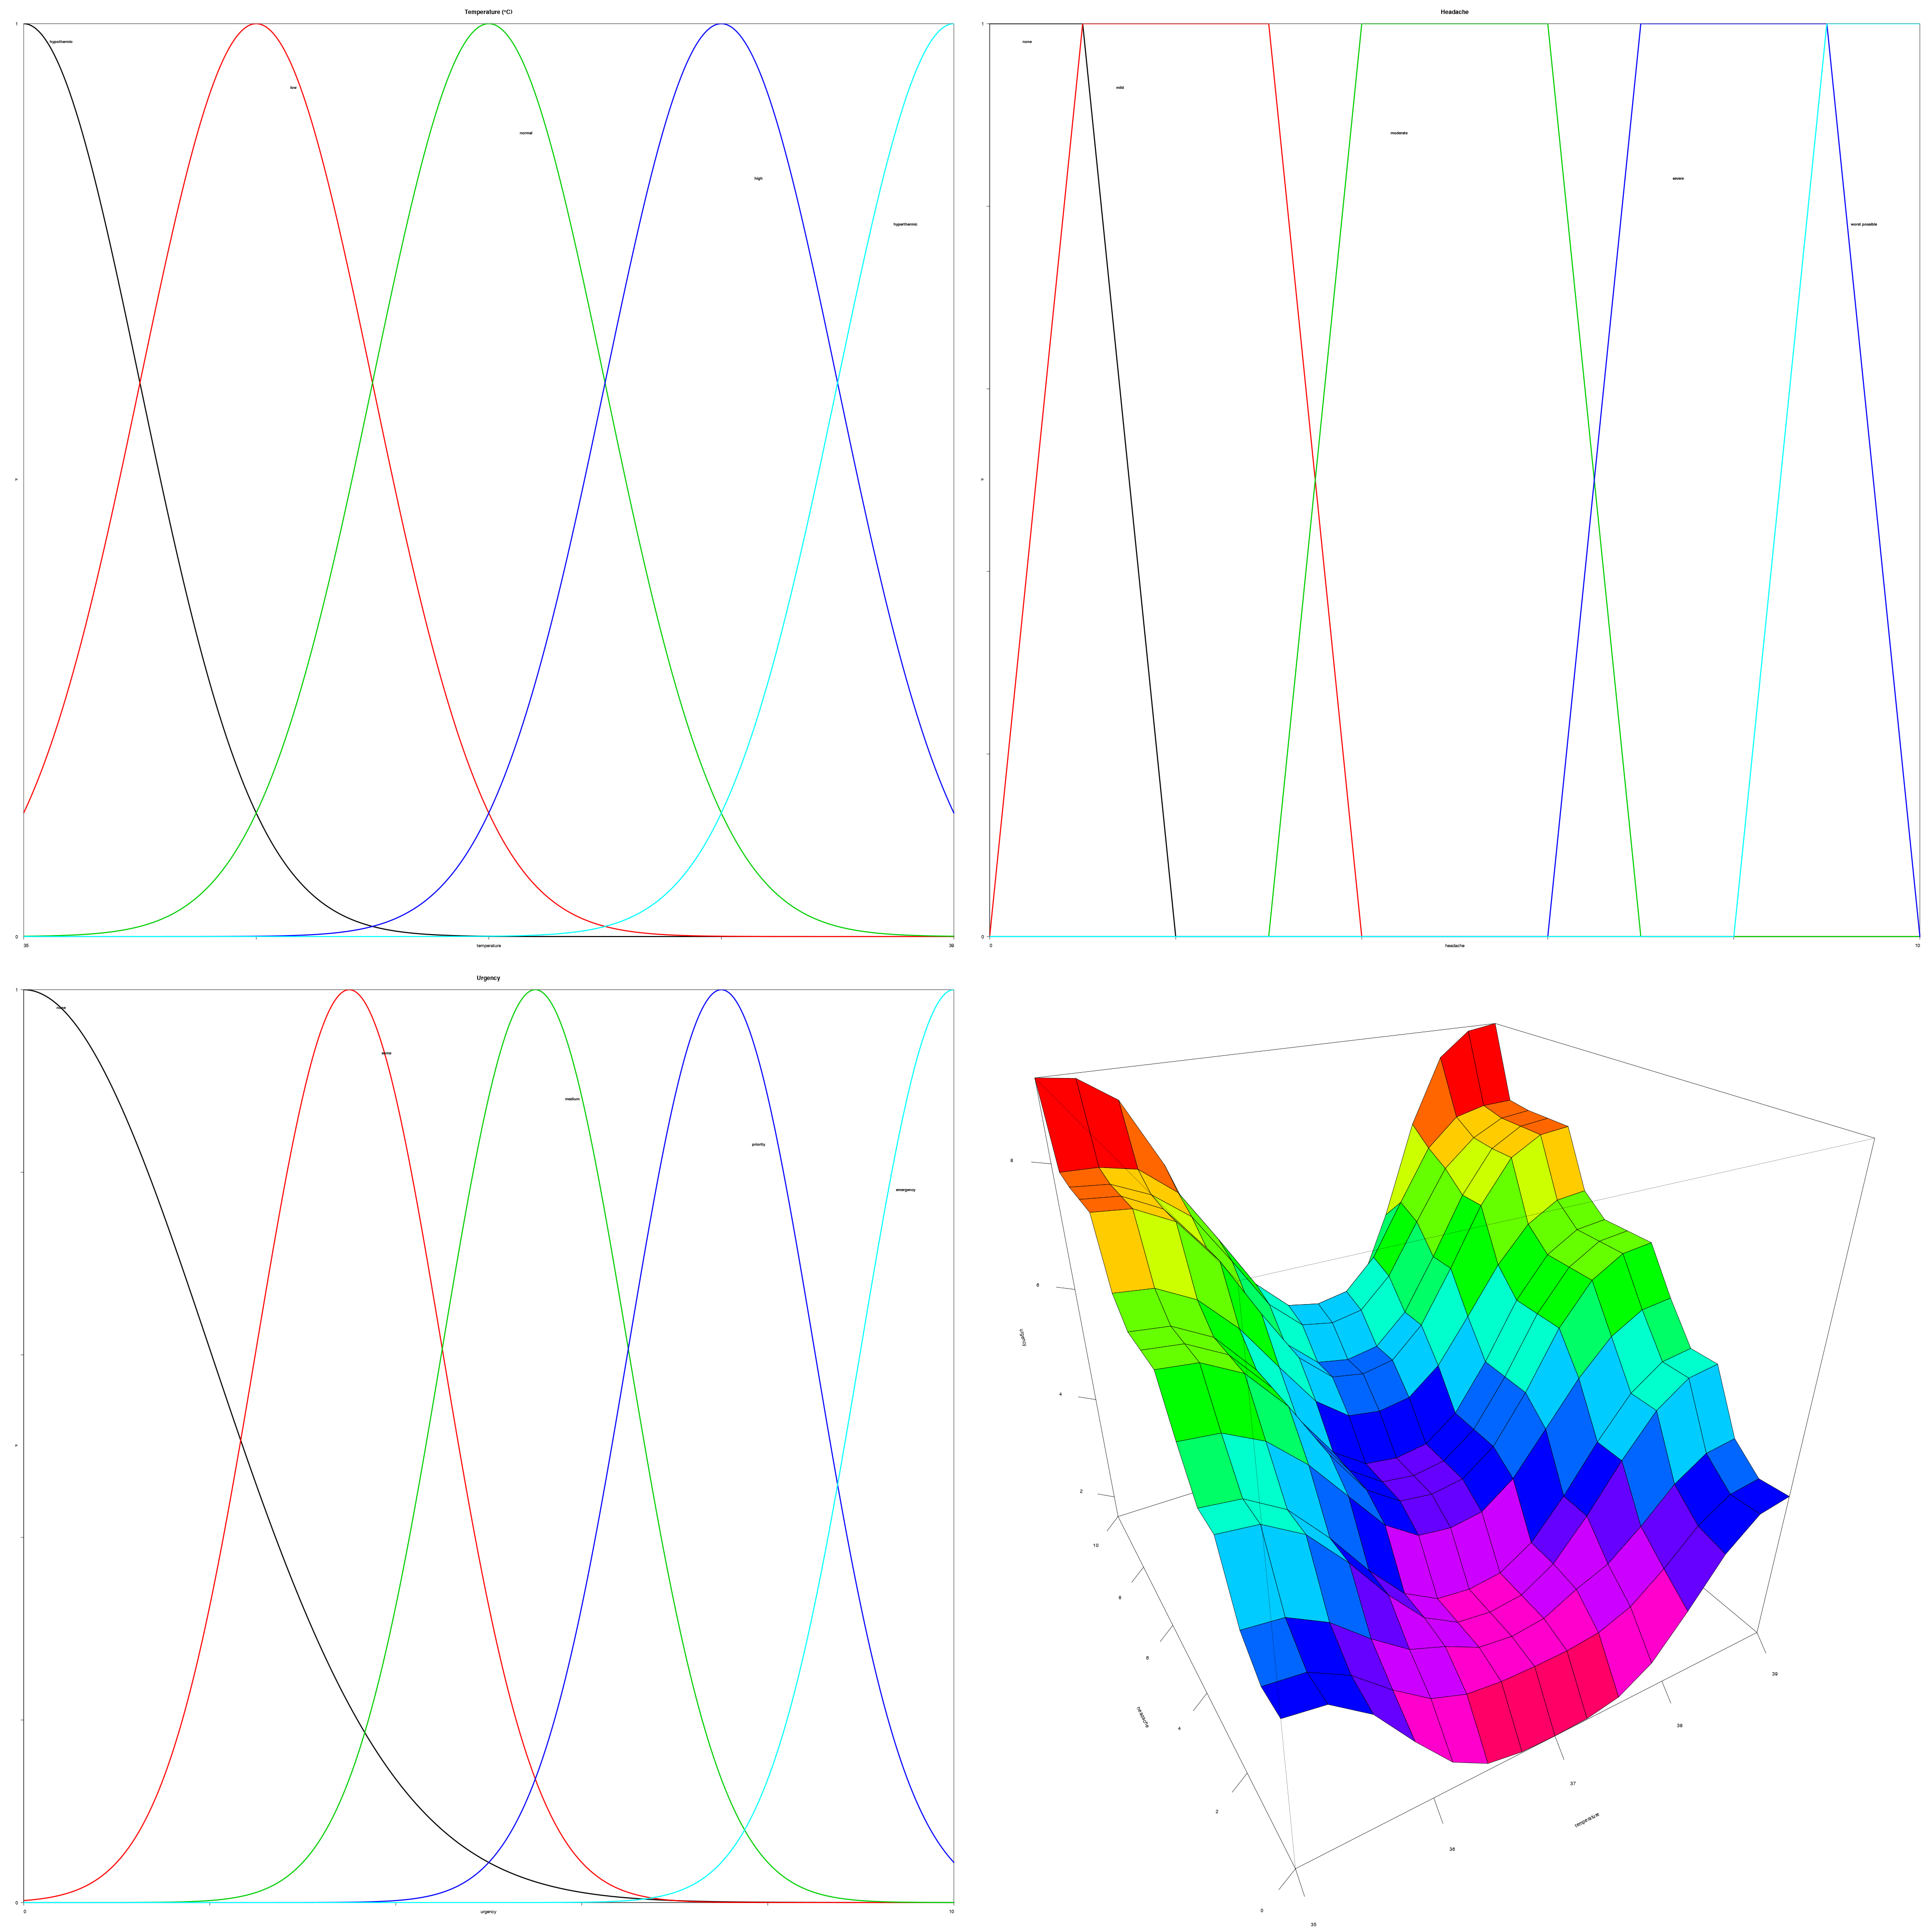
\includegraphics[width=0.4\textheight]{membershipFns03.png}
  \label{fig:membershipfns3}
\end{figure}

\begin{figure}[ht]
  \centering
  \caption{FIS 4}
  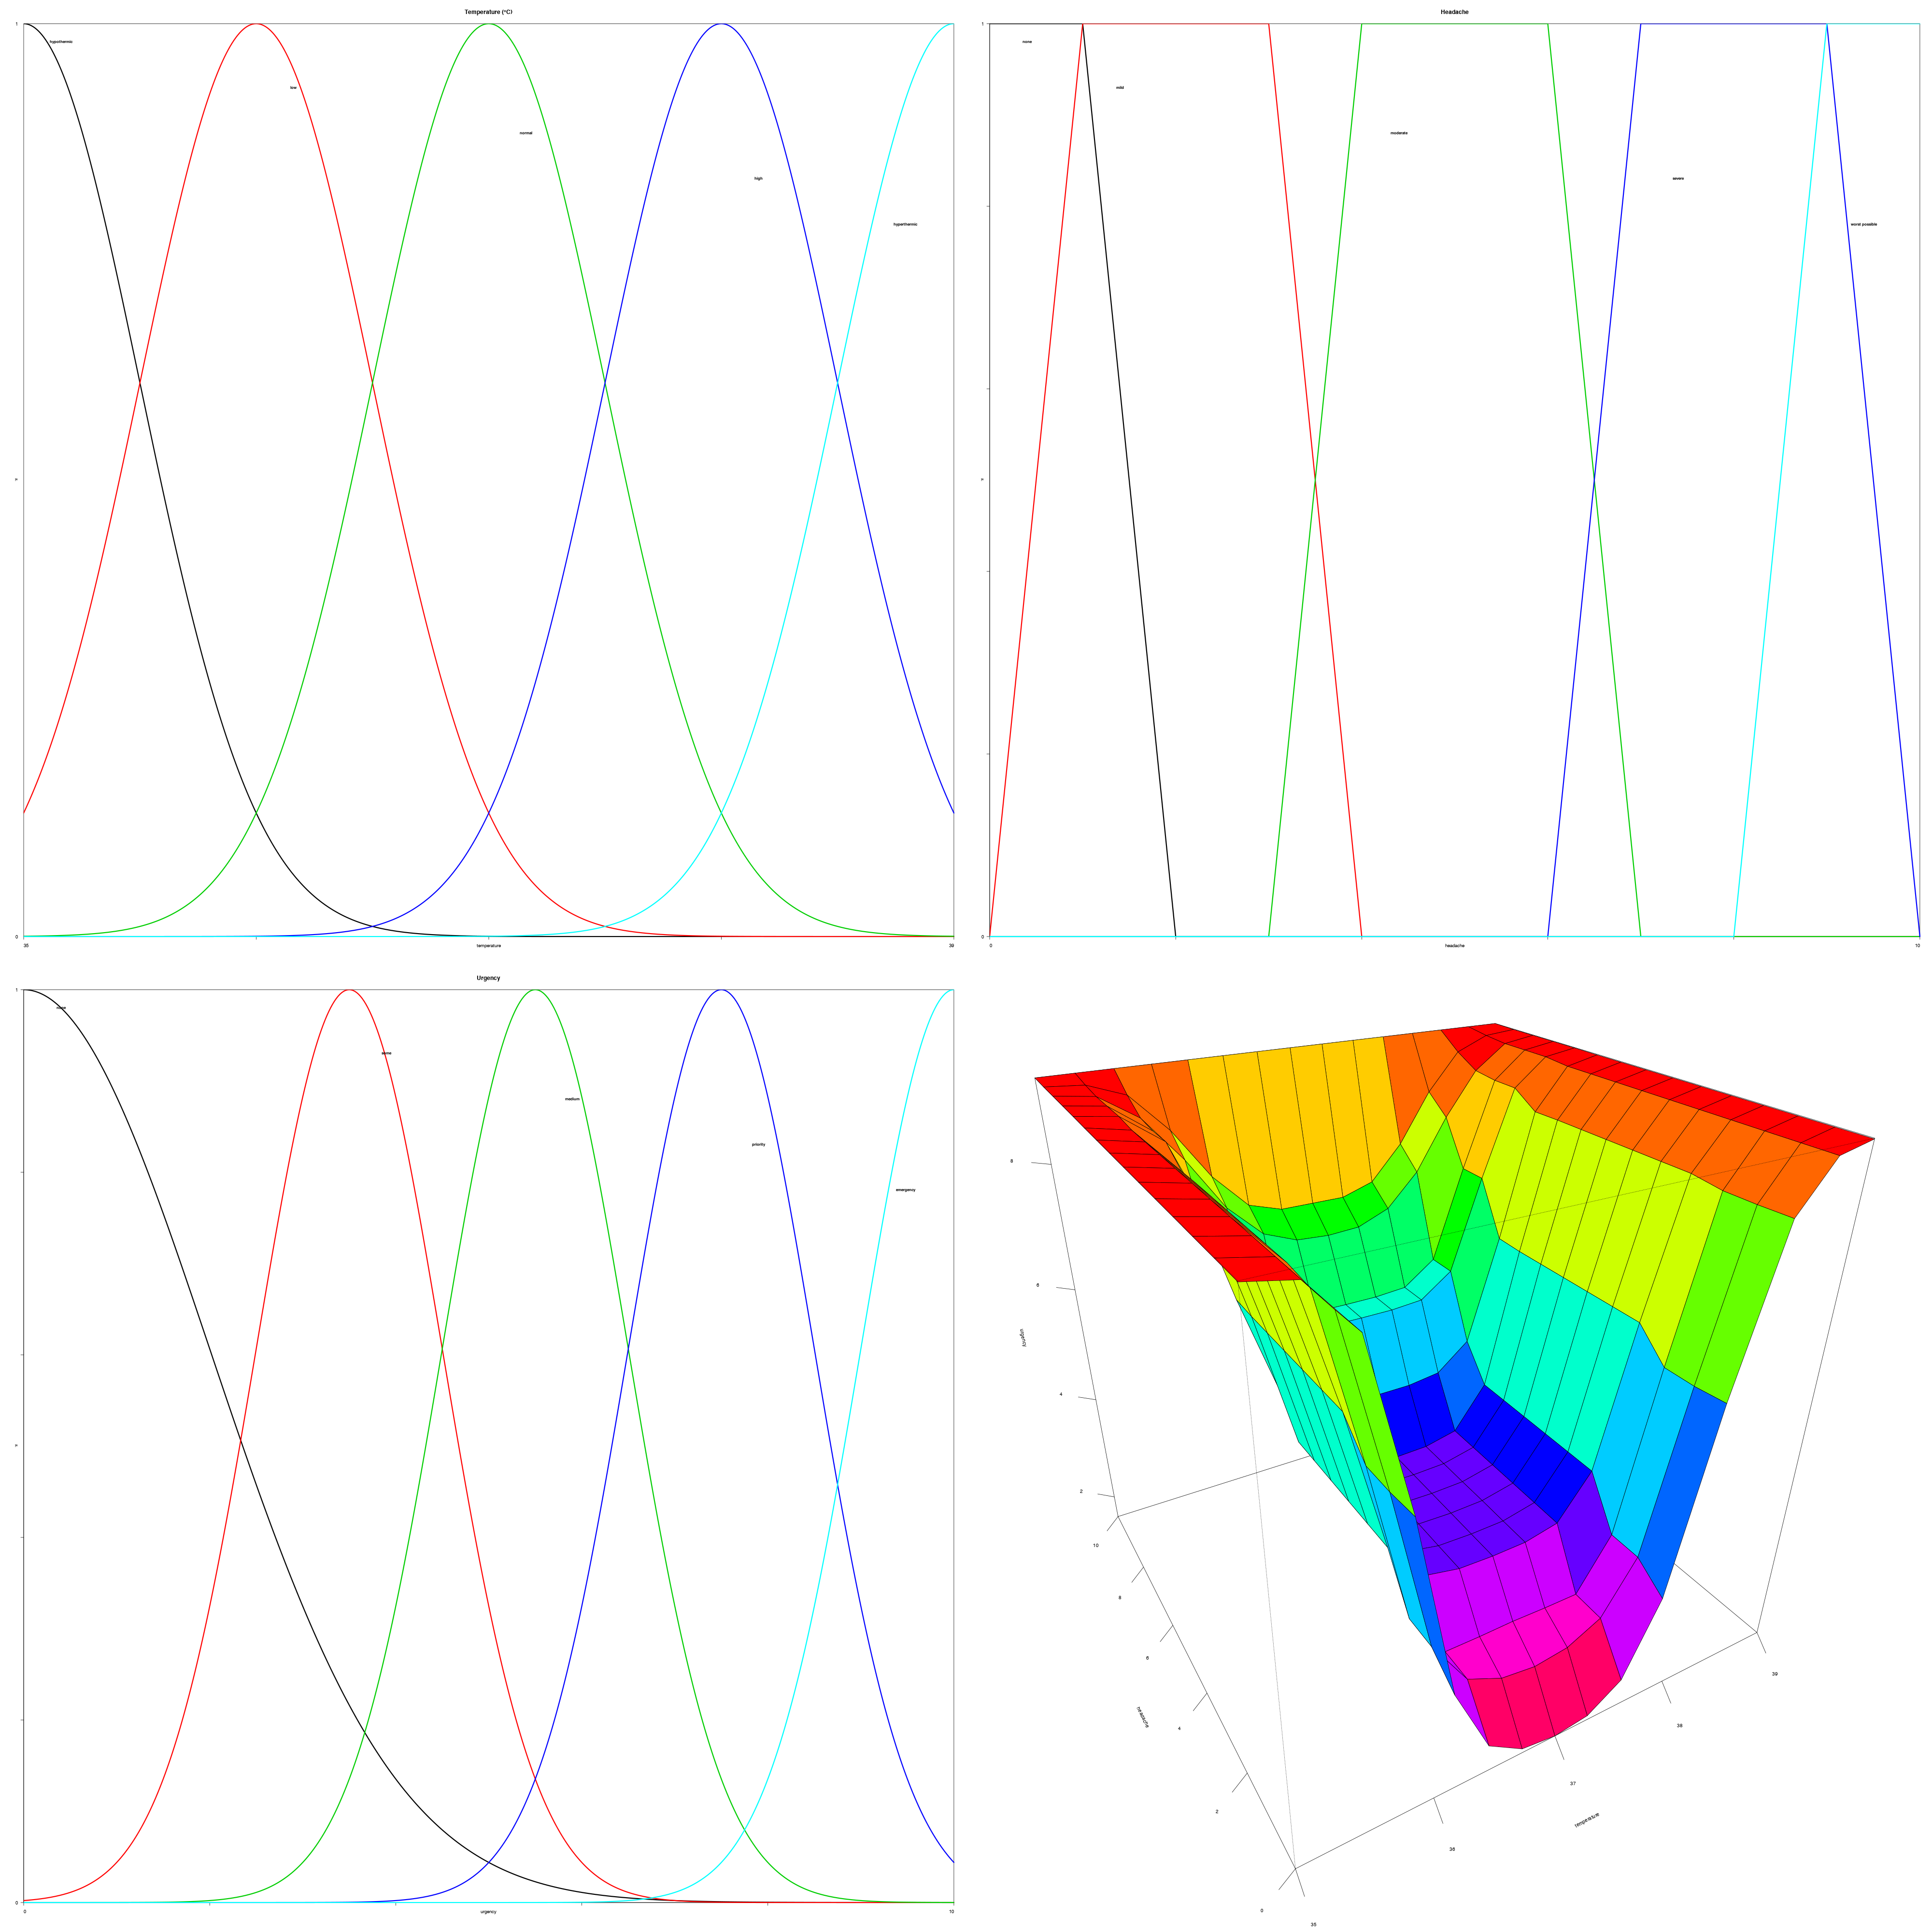
\includegraphics[width=0.4\textheight]{membershipFns04.png}
  \label{fig:membershipfns4}
\end{figure}

\begin{figure}[ht]
  \centering
  \caption{FIS 6, utilising \emph{Small of Maxima}}
  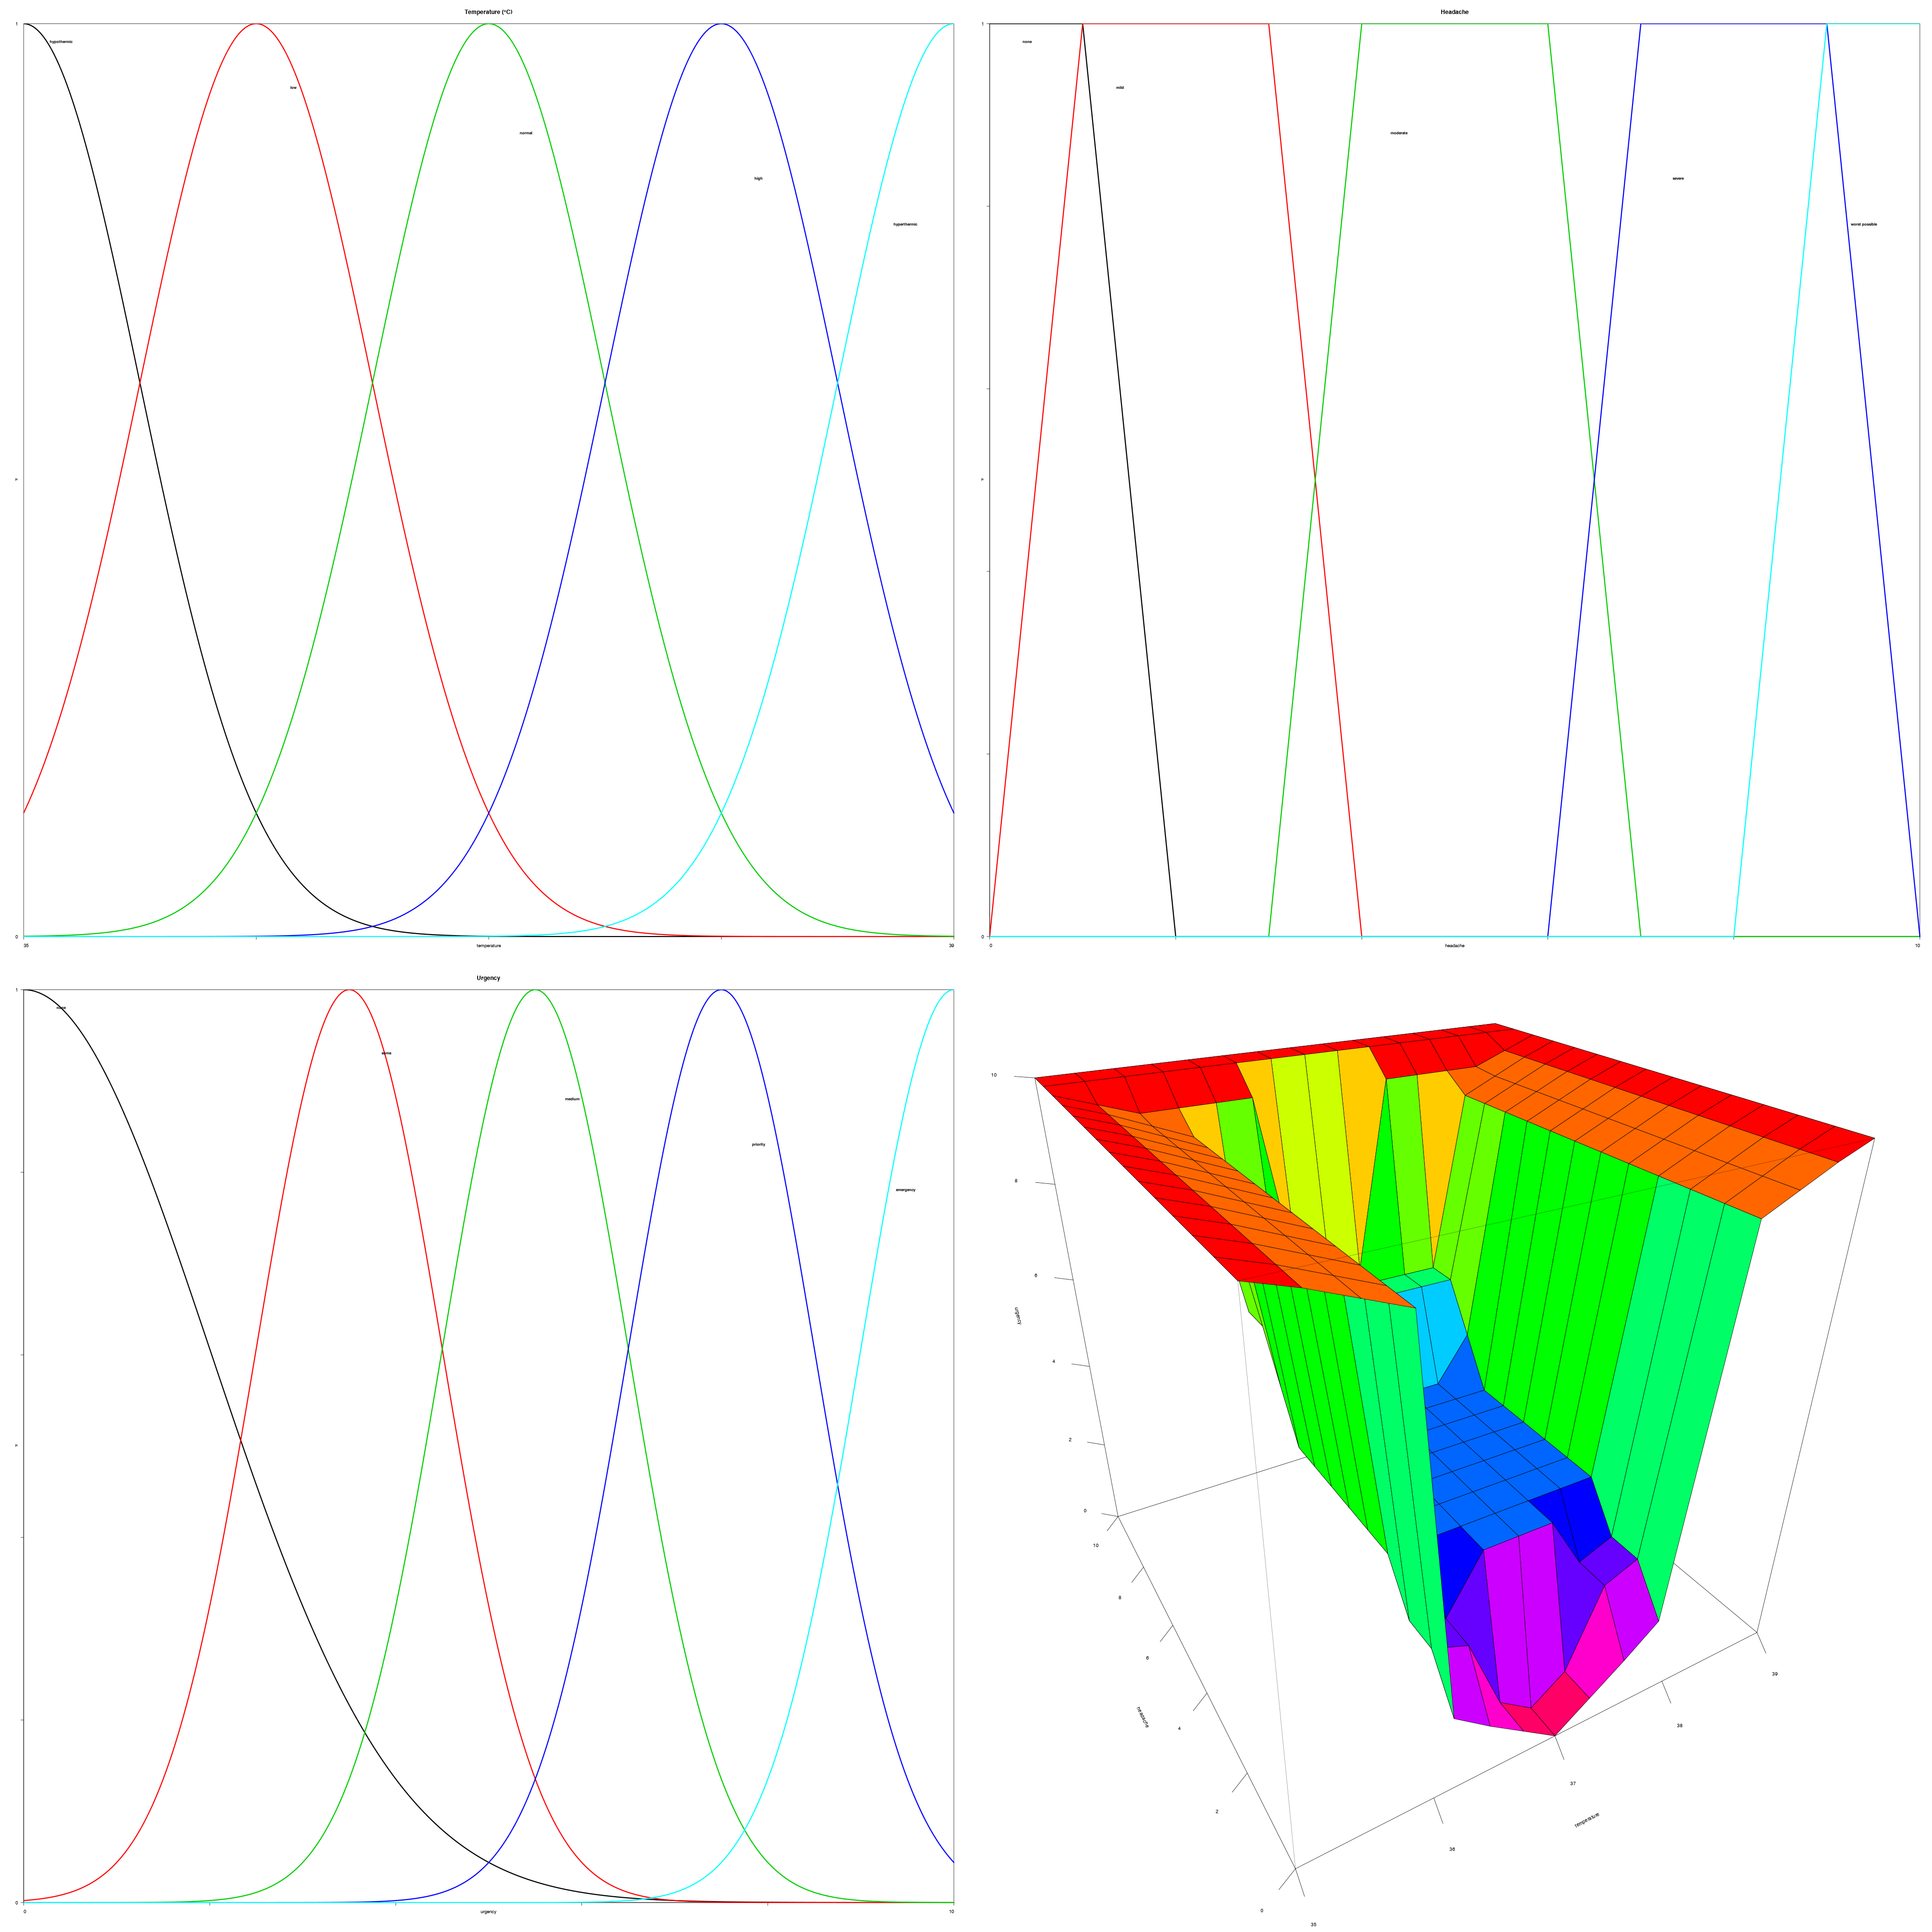
\includegraphics[width=0.4\textheight]{membershipFns06.png}
  \label{fig:membershipfns6}
\end{figure}

\begin{figure}[ht]
  \centering
  \caption{FIS 10}
  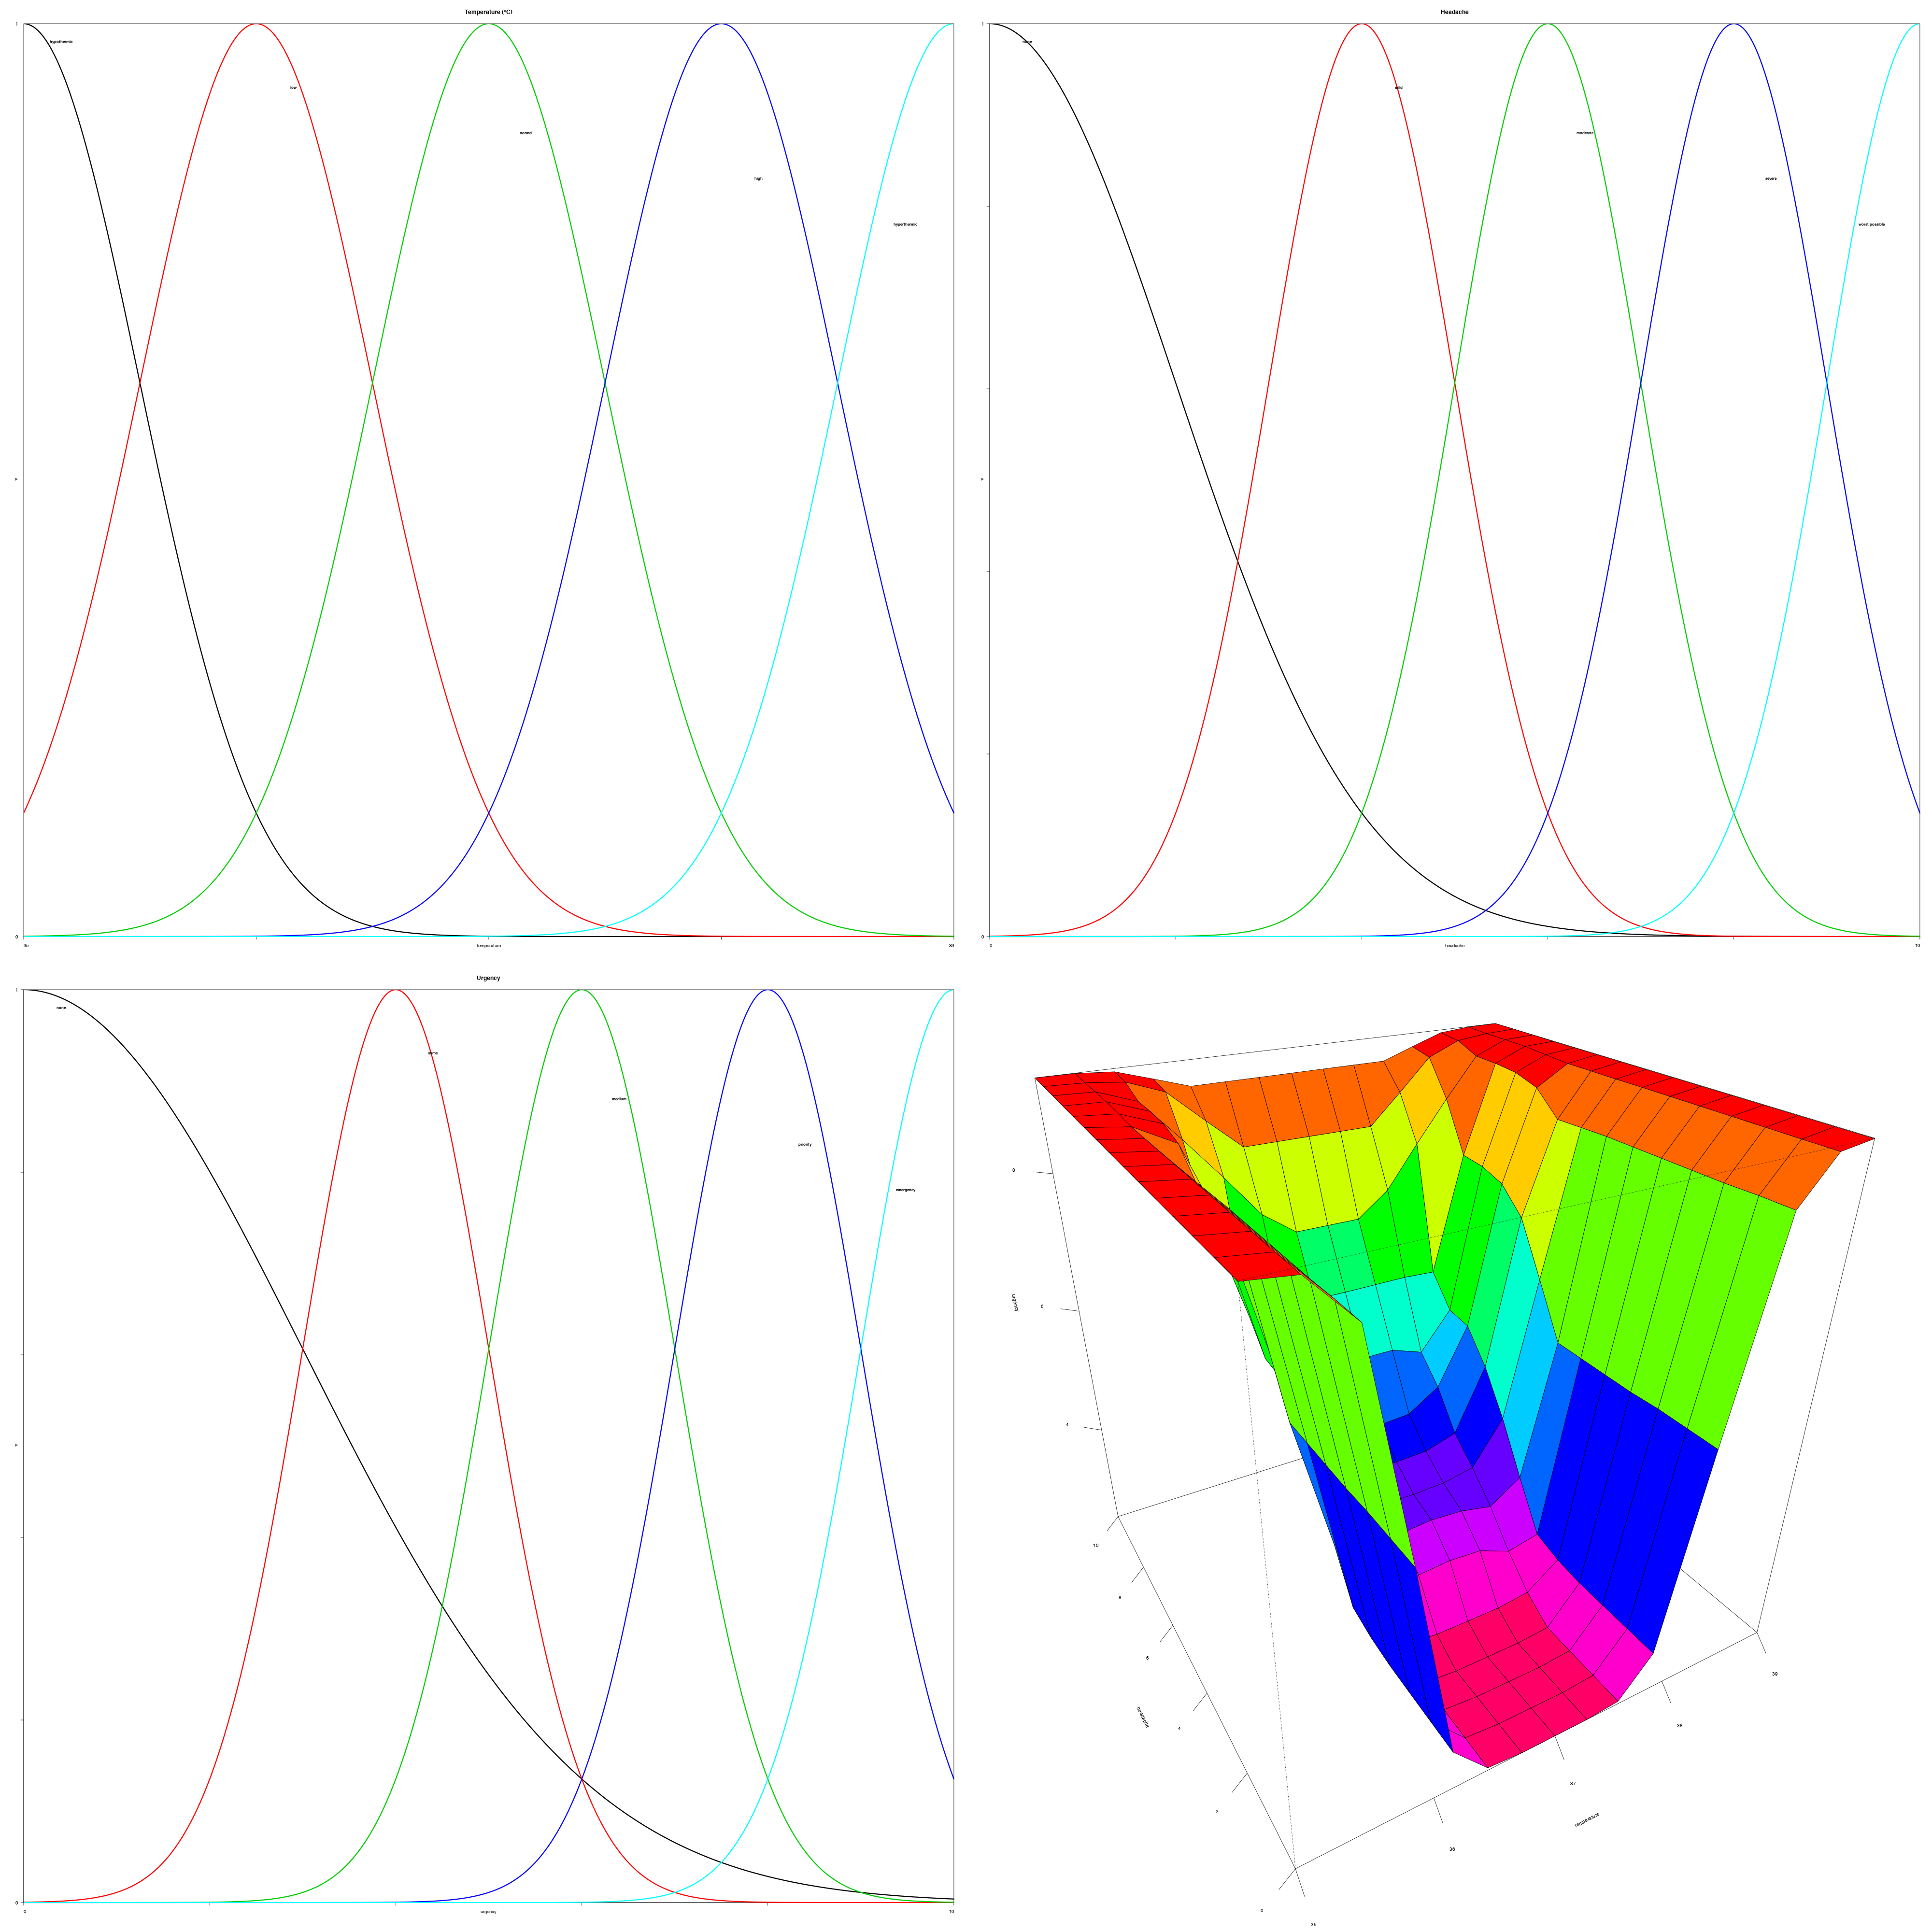
\includegraphics[width=0.4\textheight]{membershipFns10.png}
  \label{fig:membershipfns10}
\end{figure}


\end{document}
